\documentclass[spanish, a4paper]{article}

\usepackage{ulem}
\hoffset=-1.9cm \voffset=-2.5cm
\parskip=0.5cm
\topmargin 1cm

\textwidth 18cm
\textheight 24cm

\usepackage{caratula}
\usepackage[spanish]{babel}
\usepackage[utf8]{inputenc}
%\usepackage[latin1]{inputenc}
\usepackage{fancyhdr} %header lindo
\usepackage{listingsutf8}
\usepackage{pdfpages} %incluir pdf

\usepackage{caption}
\usepackage{subcaption}

\providecommand{\keywords}[1]{\textbf{\textit{Palabras Clave ---}} \textit{#1}}

\usepackage{color}

\definecolor{dkgreen}{rgb}{0,0.6,0}
\definecolor{gray}{rgb}{0.5,0.5,0.5}
\definecolor{mauve}{rgb}{0.58,0,0.82}

\lstset{inputencoding=utf8/latin1}
\lstset{
  frame=none,
  xleftmargin=0.1in,
  stepnumber=1,
  numbers=left,
%  numbersep=5pt,
  numberstyle=\ttfamily\tiny\color[gray]{0.3},
  belowcaptionskip=\bigskipamount,
  captionpos=b,
  escapeinside={*'}{'*},
%  language=Prolog,
  tabsize=1,
%  emphstyle={\bf},
%  commentstyle=\it,
%  stringstyle=\mdseries\rmfamily,
  showspaces=false,
%  keywordstyle=\bfseries\rmfamily,
%  columns=flexible,
%  basicstyle=\small\scriptsize,
  showstringspaces=false,
  morecomment=[l]\%,
}


\pagestyle{fancy}
\lhead{Teoría de Lenguajes}
\rhead{1C 2017}

\newcommand{\persona}[1]{\underline{#1}}

\begin{document}

\fecha{\today}
\titulo{Analizador Sintáctico y Semántico para $\lambda^{bn}$}
\materia{Teoría de Lenguajes}
%\submateria{asd}

\integrante{Gabriel Eric Thibeault}{114/13}{gabriel.eric.thibeault@gmail.com}
\integrante{Gonzalo Ciruelos Rodríguez}{063/14}{Gonzalo.ciruelos@gmail.com}
\integrante{Luis Agustín Nieto}{46/01}{lnieto@dc.uba.ar}

\maketitle

%\tableofcontents

\newpage
\section{Introducción}
\section{Gramática}
$$ E \rightarrow S L | S  $$
$$ S \rightarrow S C   | \lambda  $$
$$ C \rightarrow (E) $$
$$ C \rightarrow var $$
$$ C \rightarrow true $$
$$ C \rightarrow false $$
$$ C \rightarrow 0 $$
$$ C \rightarrow iszero(E) $$
$$ C \rightarrow succ(E) $$
$$ C \rightarrow pred(E) $$
$$ C \rightarrow if E else E then C $$
$$ L \rightarrow \ V : T . E $$
$$ T \rightarrow T' -> T $$
$$ T \rightarrow T' $$
$$ T' \rightarrow (T -> T') $$
$$ T' \rightarrow Bool $$
$$ T' \rightarrow Nat $$


\section{Código}
\subsection{lexer.py}
\lstinputlisting[language=Python,label=tipos]{../lambda_calculus/lexer.py}      
\newpage
\subsection{parser.py}
\lstinputlisting[language=Python,label=tipos]{../lambda_calculus/parser.py}      

%hay que arreglar lo de la numeracion
%\newpage
%\setboolean{@twoside}{false}
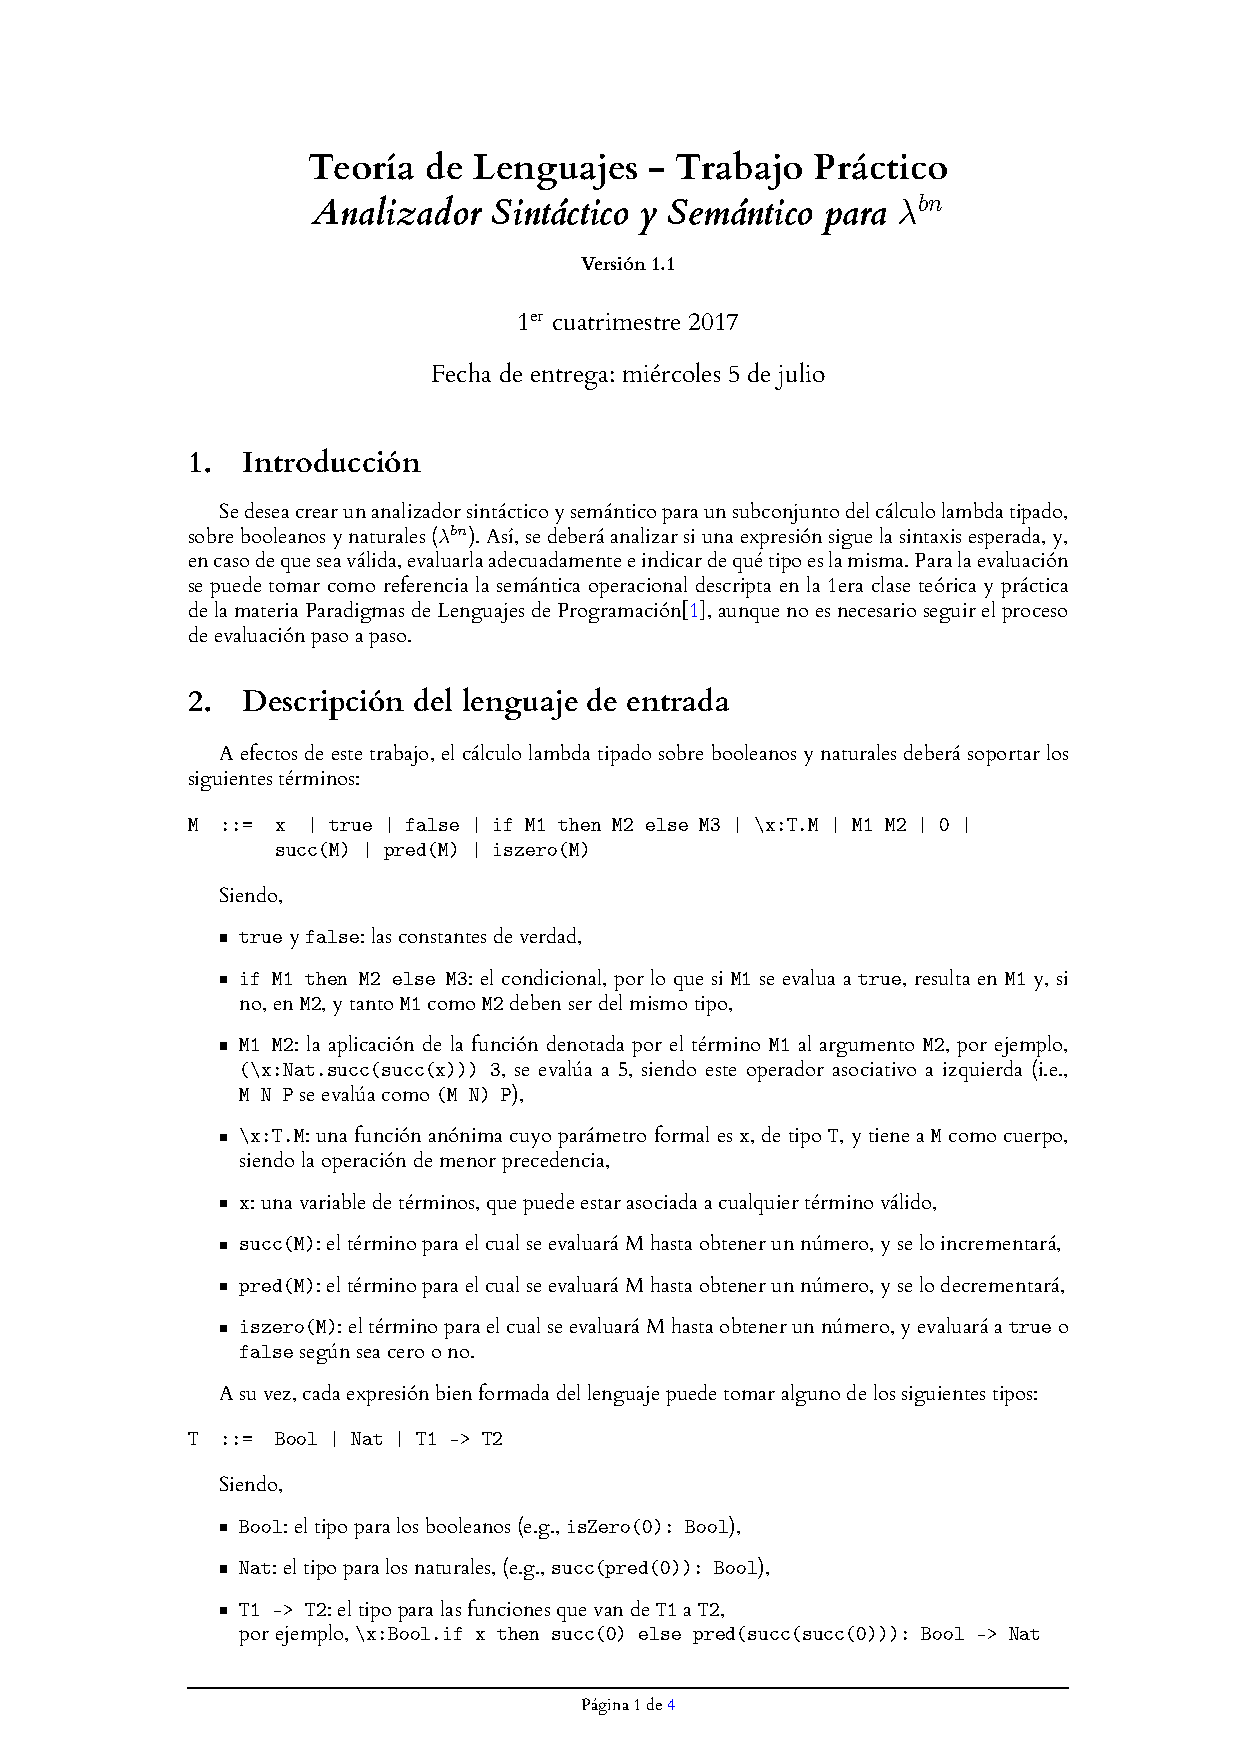
\includepdf[pages={1},pagecommand=\section{Enunciado},offset=40 -75]{enunciado.pdf}
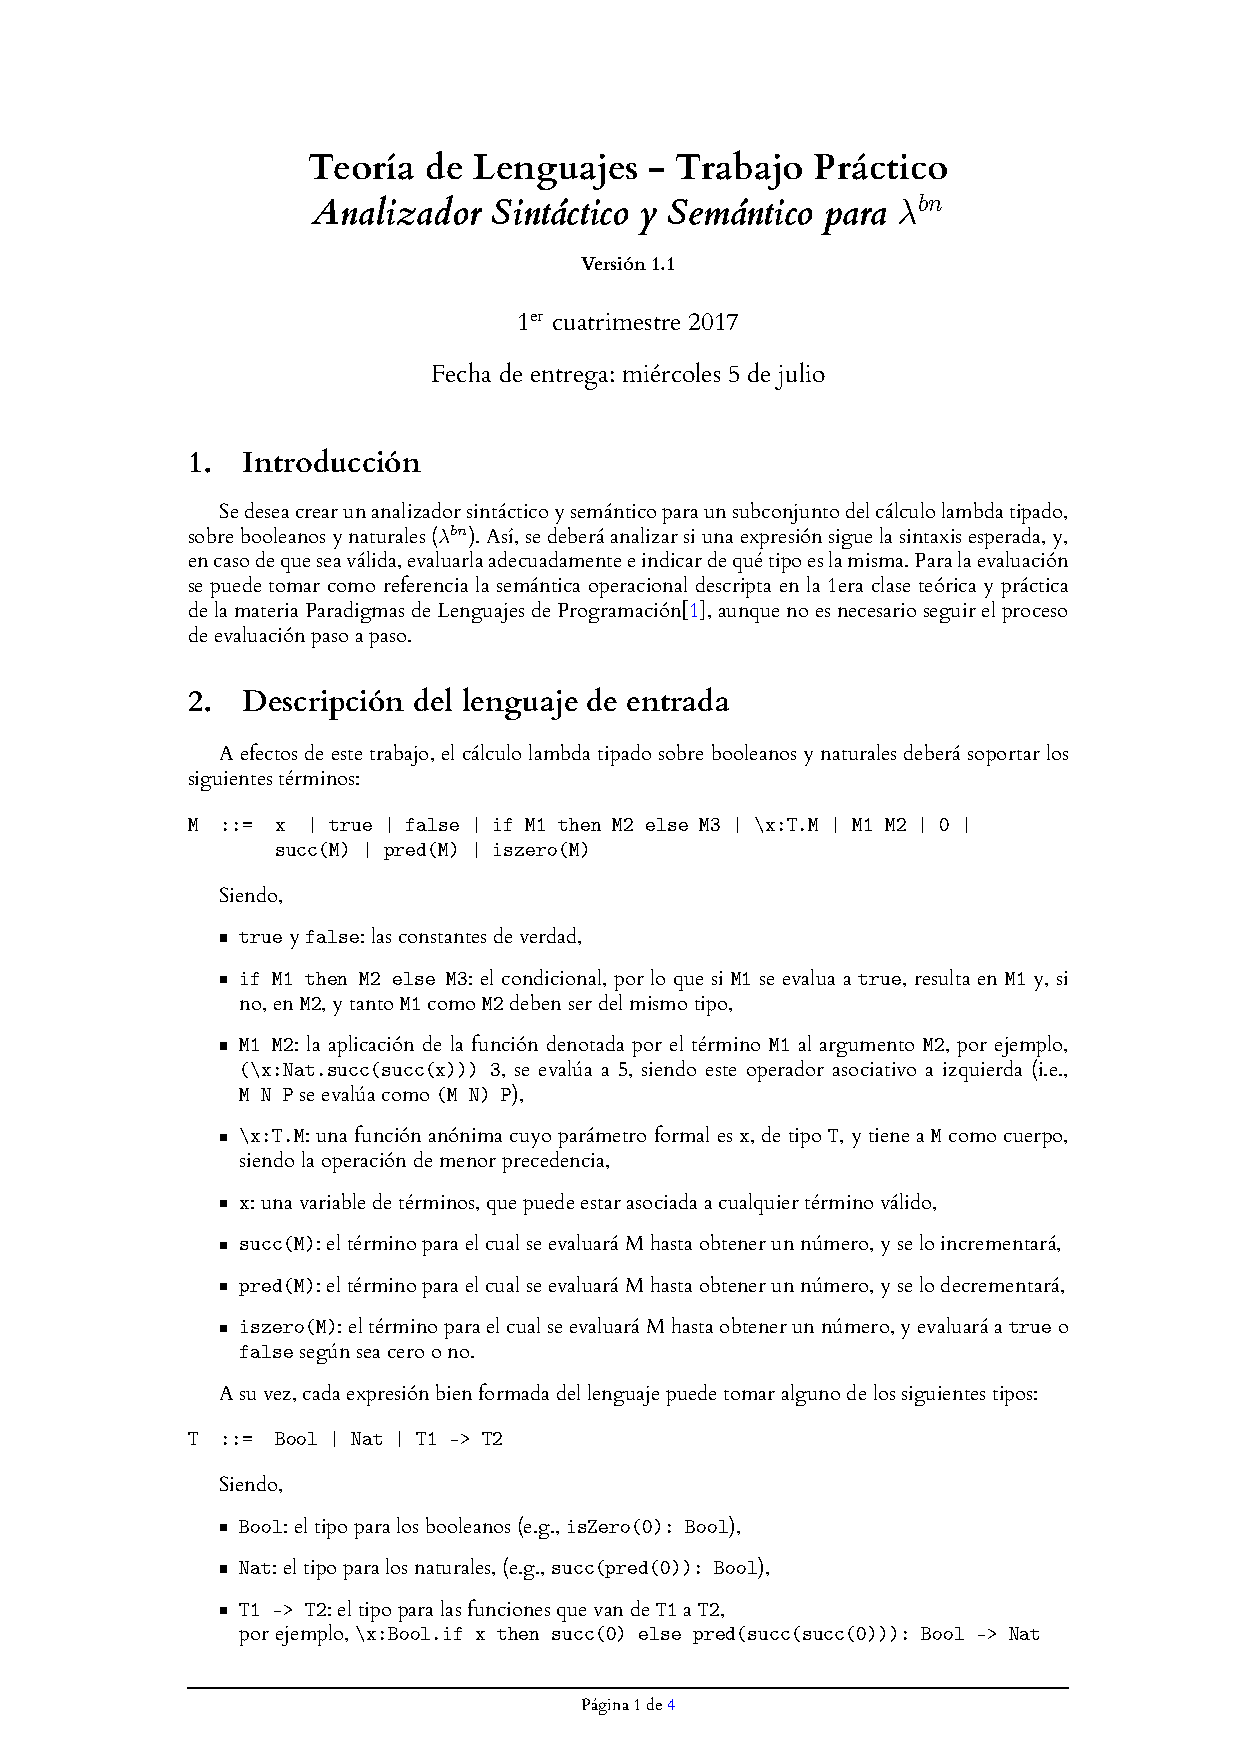
\includepdf[pages={1,2,3,4},offset=40 -75]{enunciado.pdf}

\end{document}
